\chapter{多版本缓存事务技术}
\label{chap:vct}

我们以当前日益重要的手机移动环境作为研究工作的载体。当前手机上的数据存储主要继承自桌面或服务器系统,采用以闪存(flash)为中心的设计:动态内存(DRAM)实质上只担负I/O缓存的角色,为速度更慢的闪存提速。为了改进手机应用带给用户的响应延迟和运行时的能量效率,本章提出了一种新的面向手机数据存储的文件系统MobiFS,它将动态内存与闪存整体视作一个非易失内存系统,采用了以内存为中心的设计。该设计不再定时向闪存回写缓存中的脏数据,也不在收到fsync()系统调用的时候冲刷数据。相反,它动态地选择合适的时机在闪存中以增量的方式生成内存中数据的检查点。生成检查点的时机由一组对应用和用户自适应的策略算法决定,以优化能量效率和应用响应度。MobiFS将原子性事务机制引入页缓存来保证系统故障时的数据一致性。本质上,该设计的权衡在于接受适度的数据滞后量来获得更好的应用响应度和能量效率,并且以定量的方式调整权衡的程度。实际测评显示,MobiFS可以实现18.8倍于安卓(Android)平台默认文件系统Ext4的写吞吐率,并能够支持11.2倍的数据库每秒钟平均事务量;常用的真实应用下,MobiFS在响应时间和能耗方面的改进分别可以达到51.6\%和35.8\%。

\section{文件系统及效能优化}

\subsection{文件系统对应用效能的影响}

优秀的应用体验决定了手机生态系统的成功。特别地,对于高度交互的手机使用场景和以电池为能源供应的手机设备,应用的响应度(responsiveness)和系统能耗成为两个新的关键需求。最近的研究工作指出,数据存储对应用体验有显著影响。存储I/O可将应用响应度减缓一个数量级~\cite{Desnoyers:2013:SRN:2534861.2534867, Kim:RSS:2012,Lee:2012:SLD:2380356.2380367, Nguyen:2014:ISR:2638728.2638841},并以直接或间接的方式影响设备能量消耗~\cite{Li:2014:EOM:2591305.2591316,Nguyen:2013:SSE:2493432.2493505,
Xu:2013:OBE:2462456.2464444}。

现在的手机软件平台主要从桌面和服务器系统继承了数据存储的设计。例如,安卓(Android)和Windows Phone分别默认使用Ext4和NTFS文件系统。然而,这些数据存储系统的设计既没有反映出手机用户的新需求,也没有充分挖掘手机使用环境的独特优势。实际上,有限数目的前台应用、日益充足的DRAM容量以及手机应用联网的内在属性等手机平台的特性,为我们提供了传统桌面和服务器系统所不具备的新的设计空间。

\subsection{现有文件系统设计和页缓存}

一个典型的文件系统包含三个主要组件:(1)服务系统调用的接口逻辑;(2)放置热点数据的缓存,通常为页缓存;(3)持久性介质的管理组件。本章工作主要涉及其中的两个部分:系统调用逻辑和页缓存。

传统文件系统通常基于POSIX~\cite{POSIX}接口实现。POSIX包含了两种方式,用于在优化I/O性能的同时减小数据的滞后量并提供对数据一致性保障机制的支持:(1)异步的写操作\texttt{write}\footnote{为防止混淆,这里的\texttt{write}仅指不传递如O\_SYNC等特殊参数的异步写调用。}将用户数据移动到页缓存中。每隔一段固定的时间(Android上默认值为5秒),脏页会被后台进程回写到闪存中。(2)同步的\texttt{fsync}系统调用立即强制刷出目标文件的数据。数据库系统通常依靠\texttt{fsync}来维护故障时数据一致性。我们以预写式日志(write-ahead logging)为例。数据库系统首先在独立的日志中记录对数据的更改,而不是直接修改主数据文件。然后,数据库对日志文件调用\texttt{fsync}。该调用成功返回,可以保证日志文件在持久化介质上的持久性。最后,数据库才将日志中记下的那些更改在主数据库文件上实际执行。

\subsection{数据一致性和滞后性}

系统故障会导致页缓存中的数据丢失,这实质上会带来两个可能的负面结果:数据不一致和数据滞后。本章的数据一致性是指\emph{时间点一致性}~\cite{point-in-time-consist},意味着持久性数据总是对应于历史上的时间点$T$,从而所有$T$之前的写都体现在持久性数据中而所有$T$之后的写都不保留。异步的写调用\texttt{write}是无法保证数据一致性的。特别地,当数据保存在页缓存中的时候,可能被后续的写覆盖或者各个不重合写的顺序被打乱。这样在系统故障的情况下,如果只有部分缓存数据被冲刷到闪存上,那么这部分数据就可能导致违背时间点一致性的要求。

与此同时,\emph{数据滞后量}对大部分面对系统故障的应用而言是一个不太关键的问题。数据滞后量是指当前内存中易失性数据与闪存中持久性数据之间的“距离”。这个距离可以从很多角度衡量,比如版本~\cite{Bailis:2012:PBS:2212351.2212359}或者时间~\cite{Ports:2010:TCA:1924943.1924963}。

\section{以内存为中心的文件系统}

在本章我们提出以内存为中心的(memory-centric)手机数据存储设计,将有电池供能的手机的DRAM视作非易失性内存的一种形式,通过传统的文件系统的接口为应用提供服务。我们从传统的以闪存为中心的(flash-centric)设计切换到以内存为中心的设计,将手机用户特别关注的能量效率和应用响应度提升为系统效能优化的首要指标。传统以闪存为中心的设计源自桌面和服务器系统,将可持久化的闪存设定为中心存储,而视DRAM为临时性的缓存介质。很多最新的优化研究~\cite{Jeong:2013:ISO:2535461.2535499, 6558430, Kim:2014:RJJ:2591305.2591332,
Nguyen:2014:ISR:2638728.2638841, Nguyen:2014:SAL:2638728.2638763,
Nguyen:2013:SSE:2493432.2493505, 6986137}依然沿用了这种传统设计思路。与此相反,我们重新审视了手机存储系统设计默认的基本假设。我们以内存为中心的设计思路将DRAM视作长期的可靠的中心存储,而将闪存视为备份或归档层。具体地,(1)现有设计中频繁的内存脏数据回写不再需要;(2)现有设计中代价较大的文件数据同步系统调用fsync()等可以集中处理和调度,避开应用I/O的关键路径。这两个改进对应用响应度和手机能量效率都可带来显著影响~\cite{Desnoyers:2013:SRN:2534861.2534867,Kim:RSS:2012, Lee:2012:SLD:2380356.2380367,Nguyen:2014:ISR:2638728.2638841}。我们选择最优的时机在闪存上增量式地生成数据的检查点(checkpoint),并根据应用行为、用户交互和设备状态等动态地调整策略。

为了操控生成检查点的时机,我们更改了POSIX接口fsync()的语义,变为非阻塞的异步调用。但某些应用以及数据库(例如SQLite)依赖于同步的fsync()来保证数据的一致性。为了解决一致性问题,我们设计了多版本缓存事务(versioned cache transaction,VCT)的机制,以保证数据在内存中保存和写出到闪存都是以原子性事务的方式进行。结合智能的检查点生成策略和多版本缓存事务,可以确保将频繁数据回写的损耗降到最低的同时数据的一致性得到保护。

为了量化地实现策略权衡,我们将“持久性”解释为一个连续变量,而不是一个二元值(“持久”或“不持久”)。直观上看,给定系统故障的概率,闪存上数据的滞后程度越小,我们可以认为总体数据的持久性越高。所以,我们使用数据滞后量作为“持久性”的一个度量。另外,我们的权衡策略还依赖于持久性和一致性在存储系统上的分离。最近的若干工作~\cite{Chidambaram:2013:OCC:2517349.2522726,
Mickens:2014:BFC:2616448.2616473}在不同领域利用了相似的分离手段,但它们没有使用以内存为中心的设计,也没有为手机应用设计优化策略——我们目前缺乏针对手机环境的系统的量化的研究。

我们基于非易失性内存假设的系统设计,主要的优势在于赋予存储系统可以针对应用和用户行为进行动态优化的自由。传统阻塞等待的\texttt{fsync}系统调用和时间间隔固定的冲刷机制都无法做到这一点,不能很好地支持对移动系统能耗和用户体验的优化。我们的观察带来了针对应用和用户的自适应的检查点生成算法。具体来说,我们回答了对哪些数据生成检查点(即写出到闪存)和何时生成检查点这两个问题。我们的方案会考虑设备状态和用户交互,对每个应用独立地确定生成检查点的最佳时机。

另一方面,非易失性内存的假设之所以能够成立,是因为以手机为代表的移动系统呈现出有利的特性。首先,手机设备是由电池自主供给能量的,所以由外部因素(如桌面和服务器系统面临的断电)导致DRAM数据丢失的风险大大降低;其次,当前手机平台由于软件系统故障死机的概率很小,只有6\%的随机调查用户遇到每个月一次以上的死机;第三,大部分手机应用都是联网的,因此本地丢失的用户数据可以从远程服务器同步找回(例如Gmail、Facebook、Twitter)。我们调研的在谷歌应用商店最为流行的62个免费应用中,只有8个对本地数据丢失敏感\footnote{对于管理诸如无法重现的照片等关键数据的应用,依然可以通过简单配置选项使用常规的文件系统功能。}(详见\ref{vct:insight}节)。

我们选择文件系统作为面向应用的接口,是出于以下三个原因:(1)文件系统支持直接的应用访问和数据库,可以允许MobiFS涵盖所有存储I/O。与此同时,我们可以允许特定应用选择性开启或关闭MobiFS的功能。(2)我们的方案不更改标准的文件系统接口形式,所以上层应用不需要更改实现。(3)我们的实现可以独立于下层闪存管理组件。例如,MobiFS可以实现与Ext4、Btrfs~\cite{Rodeh:2013:BLB:2501620.2501623}或者最新的F2FS~\cite{188454}的整合。

总之,我们的文件系统MobiFS实现了如下三个贡献:(1)构建了以内存为中心的移动存储设计,赋予手机内存非易失的属性,论证了其可行性和重要性。(2)提出了多版本缓存事务机制,将原子性事务引入传统操作系统页缓存,以保证数据在内存和闪存上的一致性。(3)在移动环境下探索了数据滞后量、能量效率和应用响应度之间的权衡,提出了一个新的指标来量化这些权衡,并且刻画了不同应用或用户的I/O访问模式;以实验数据为基础,设计了策略框架来平衡不同的元素。(4)我们在Android上实现了可用的原型系统,包含整合Ext4和Btrfs的两个版本。基于真实应用和用户的测评显示,我们的系统与Android上默认的Ext4文件系统相比,可节约高达35.8\%的能量消耗,提升高达51.6\%的应用响应度;还实现了18.8倍的文件写吞吐和11.2倍的数据库事务吞吐。

\subsection{设计原理}
\label{vct:insight}

我们以内存为中心的文件系统设计是基于如下五条基本原则和假设。这些原理针对我们以能耗和响应度为优化目标的手机应用环境,并以实验或数据观察为基础。

\textbf{原理1} 当前手机内存DRAM的容量足够支持应用数据存储。

手机内存DRAM的容量经历了快速的增长(自2010年以来8倍增长,从512~MB到4~GB),当前标配已达到2~GB或更多。而该DRAM大小已经可以支持在桌面电脑上运行Windows XP系统。尽管手机应用的数据量需求也在增长,但其增长率相对较低。我们以网页请求的大小为例,其自2010年以来的同期增长率仅为94\%~\cite{HTTP:Transfer:2013}。此外,手机环境下限于屏幕大小,用户通常只使用一两个应用,活跃的数据量有限。进一步的评测参见\ref{vct:mem-fp}节。

\textbf{原理2} 手机内存可以被视作可靠的数据存储。

首先,手机DRAM配有电池供给。此类有电池支持的内存(battery-backed RAM,BBRAM)在早期桌面和服务器配置中即被视作可靠的存储~\cite{DeWitt:1984:ITM:602259.602261, Wang:2002:CBP:647057.713872, Wu:1994:ENM:195473.195506}。其次,当前手机软件的可靠性较高,因为系统死机造成内存数据丢失的情况非常罕见。这个观察基于我们关于手机系统死机(非应用故障)频率的在线用户调查。在所有参加调查的117名手机用户中,只有6\%的用户遇到系统死机的频率超过每个月1次,而所有用户平均的死机频率只有每7.2个月一次。最后,现在大多数应用的数据会同时保存在云中或同步到其在线服务,即使本地丢失仍可复原。

我们对谷歌应用商店Google Play中流行度排行前62名\footnote{该数字为包含前50名应用同时涵盖所有分类}的免费应用进行了详细的案例研究,结果很好地支持上述最后一点结论。典型的一类应用,随时与其在线服务器保持同步,例如Facebook、谷歌地图(Google Maps)、Glide视频短信(video texting)、Fitbit以及大部分游戏(同样适用于苹果平台上的游戏中心Game Center)。另一类典型应用,完全或主要依赖本地存储,如WhatsApp(出于隐私保护不在服务器保留短信)和办公软件Polaris Office。这些应用的数据在写入闪存前有较高丢失风险。与此同时,还有一些应用介于这两类极端之间。例如,Skype在服务器上保留用户短信“30到90天”以便于在用户的不同设备间进行同步。这种情形下,由于单一手机设备问题造成数据丢失的风险几乎可以忽略。

总体来看,只有8个应用被算作数据丢失高风险的应用。这些应用如果启用MobiFS,系统死机确有可能造成用户可见的数据损失,影响用户体验。但用户或开发者可以灵活地配置应用是启用MobiFS还是使用传统的文件系统。注意,对于这些少数例外的处理,只是增加了很少的配置负担,而不是编程或开发负担。根据我们的经验,应用级别的配置选项比强制开发者使用特定编程接口或参数更加现实和易用。

\textbf{原理3} 减少写出到闪存的数据量对节约应用I/O能耗至关重要。

首先,写出操作的能耗占据应用I/O能耗的主体。前人的工作~\cite{Carroll:2010:APC:1855840.1855861}已经指出,对于相同的数据量,从闪存读入消耗的能量只有写出到闪存消耗能量的1/6。与此同时,我们对谷歌应用商店Google Play排名前十的应用进行了系统调用层的日志追踪,发现它们读入数据量平均只有写出数据量的41\%。综合可知,手机上平均而言,读闪存的能耗预计只占写闪存能耗的6.3\%。

其次,写出的数据量,而非写出的次数,是影响能耗的主要因素。在一台三星手机上进行的实验中,我们按4~MB到40~MB为单位分批次写出总共40~MB数据,通过比较发现,各组净能耗差别只有1.5\%。另外,系统待机时间不是写出数据的最佳时间,因为写出数据涉及的系统能耗有些可以在设备活跃时被均摊。根据我们的评测,在待机时冲刷数据会带来多达129\%的额外能耗。

综上所述,考虑到应用写操作的数据量本身是外部决定因素,我们优化的重点是多少原本需要写出的数据可以通过覆写而减少。数据覆写的比率可以作为能量效率的一个代表指标。

\textbf{原理4} 数据冲刷的时间对应用响应度至关重要。

数据冲刷对应用响应度的影响体现在两方面:(1)当冲刷由系统调用fsync()触发时,应用需要阻塞等待数据写出到闪存。这种情况发生频繁~\cite{Jeong:2013:ISO:2535461.2535499,Lee:2012:SLD:2380356.2380367},因为数据库依赖于fsync()。(2)当冲刷由后台回写线程触发时,它会与前台应用争抢CPU计算资源和其他资源,带来负面影响~\cite{Kim:RSS:2012, Nguyen:2014:ISR:2638728.2638841}。

不论哪种情况,数据冲刷的时机非常重要:如果冲刷可以避免阻塞fsync()的过程并且避开用户行为或CPU使用高峰,那么它对应用响应度的负面影响就可以降到最低。我们以内存为中心的设计原则利用了这一点。

\begin{figure}
  \centering
  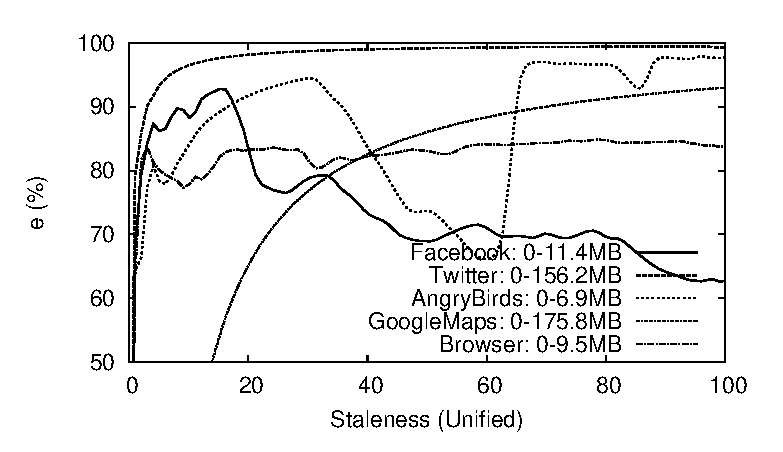
\includegraphics[width=0.9\textwidth]{e-curve-app}
  \caption{不同形状的$e$曲线表明特定于应用的I/O模式。图中数据滞后量的范围统一到0至100,实际数值标记在应用名称旁。}
  \label{fig:e-curve-app}
\end{figure}

\textbf{原理5} 应用或用户特定的I/O访问模式需要动态的量化的策略设计,以在能耗和数据滞后量之间进行权衡和优化。

不同应用或用户的I/O访问模式差别很大。我们基于三个步骤来量化这种差异以及关键的权衡:(1)我们定义了适合我们上下文的数据滞后量指标。传统数据滞后量的定义或是基于时间~\cite{Ports:2010:TCA:1924943.1924963}或是基于版本~\cite{Bailis:2012:PBS:2212351.2212359},但是基于时间的定义很难与能量效率相联系,而常规文件系统中并没有对数据版本的严格定义。为此,我们定义了新的数据滞后量指标$s$为应用自上次生成检查点以来累计写操作的数据总量。如果应用在同一个地址上先后两次写了某个单位数据量,那么数据滞后量$s$增加两个单位量,而不是一个(在这个意义上,与传统基于版本的定义类似)。(2)基于上述原理3,我们定义能量效率比$e=o/s$,其中$o$是应用自上次生成检查点以来累计覆写的数据量。因为$o<s$,$e$的取值范围在$[0,1)$内。较大的$e$值意味着,对于相同的数据冲刷量,被覆写的数据较多,也就是节约的能耗较多。(3)基于上面两个定义,我们描绘$s$上的$e$曲线来表现增加数据滞后量带来的能量效率的变化。如图~\ref{fig:e-curve-app}所示,不同应用的$e$曲线呈现不同的形状,反映出对于不同应用最佳冲刷时间会有所不同(亦适用于不同用户)。理想状况下,应用的内存数据应该在$e$曲线达到峰值时进行冲刷,写入闪存。

\subsection{系统架构}

\begin{figure}
  \centering
  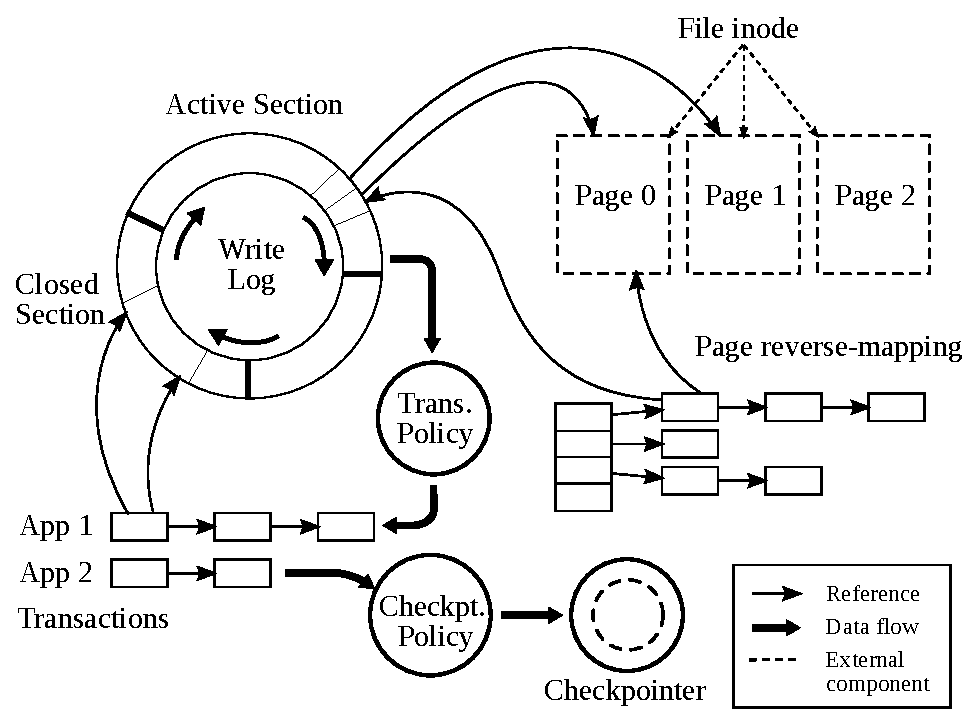
\includegraphics[width=0.8\textwidth]{arch}
  \caption{MobiFS系统架构图}
  \label{fig:arch}
\end{figure}

MobiFS主要由五个模块构成:(1)页缓存,负责在内存中存储文件数据;(2)写日志,负责维护写操作的历史,由按序排列的许多记录项构成,每个记录项会引用一个页缓存中的物理页;(3)事务,写日志中的若干记录项归并为一组,它们的一致性不受覆写和重排序等优化的影响;(4)检查点生成器(checkpointer),负责调用底层闪存管理组件以原子性方式完成事务的持久化;(5)策略引擎,负责依据优化算法划分事务的边界,监听用户交互行为,并决定生成检查点的事务和时机。图~\ref{fig:arch} 描绘了MobiFS的系统架构。

MobiFS的设计充分考虑了与现有操作系统(Linux)的兼容和组件重用。它与操作系统共享现有的页缓存结构。对于页缓存的每个写操作,都会记入写日志,通常体现为在当前事务中(写日志的末尾)追加一个记录项,除非当前事务已经包含目标页地址的记录项。为此,我们需要维护一组从页地址到写日志项的逆向映射,以判断目标页地址是否已经存在于事务中。基于写日志和逆向映射,MobiFS建立起原子性事务机制。每个事务定义了可以进行覆写和重排序等优化的一个特定范围。最终,策略引擎指导检查点生成器保存事务到闪存,同时不影响用户交互。策略引擎根据每个手机应用甚至是用户的行为及其统计指标,做出动态的智能的判断。

在一个典型的配置中,不同手机应用会拥有自己独立的写日志和事务,但它们共享逆向映射、策略引擎和检查点生成器等组件。

\section{多版本缓存事务技术}

在写日志中,可能同时引用逻辑上同一个缓冲区页的多个物理版本。多版本缓存事务用来管理这种关系。覆写和重排序等优化手段只允许用于单个多版本缓存事务内部。由于检查点生成器可保证一个事务整体的持久化和原子性,这些优化不会导致闪存数据的任何不一致状态。

\subsection{写日志}

写日志是应用所有写操作按时间排列的历史记录。写日志包含两个段:活跃段(active section)处在写日志的末尾,新的记录项会被插入活跃段;闭合段(closed section)则包含准备生成检查点的记录项。 
 
在Android平台上,一份写日志的范围涵盖一个手机应用访问的所有目录。手机应用可能使用数据库SQLite保存数据,而SQLite是一个嵌入式数据库,它与每个应用捆绑的相关文件也需要托管给MobiFS,包含在应用的写日志范围内。
 
我们之所以能够面向特定应用进行写优化,一个重要原因在于手机应用的数据路径是静态的和相互隔离的,从而避免了应用间的一致性问题。当然,的确存在多个应用共享文件数据的情况,例如文件浏览器和相册应用可能同时管理照片存放的目录。这种情况下,相关应用需要在程序逻辑层面进行处理。即便不使用MobiFS,在现有Android的文件系统上,应用同样需要处理这类情况(例如,用户通过文件浏览器手动删除了相册中原本可见的照片)。 

\subsection{事务和版本}

一个多版本缓存事务在其生命周期内经历三个状态:(1)当处于打开状态时,一个事务接收新的记录项,而这些记录项构成写日志中的活跃段。(2)当进入闭合状态时,该事务的所有记录项不再可以更改,转入写日志的闭合段。从打开状态到闭合状态的转换是单向的,不可逆的。(3)当进入提交状态时,该事务所有记录项对应的物理缓存页被检查点生成器原子性地刷出到闪存。成功提交之后,该事务及其记录项即从写日志中消除。 
 
当一个写操作到达时,MobiFS需要处理三种情况:(1)如果要写入的目标页不存在于逆向映射中,那么意味着写操作将进入一个未被写日志涵盖的页。MobiFS会在写日志中追加一个记录项,建立到缓存页的映射,并建立逆向映射。(2)如果逆向映射已经存在且指向一个写日志闭合段中的记录项,那么意味着写操作想要写入一个被保护的只读的事务。为此MobiFS对目标页执行写时拷贝(copy-on-write),并为新的页副本添加写日志记录项及映射/逆向映射。(3)如果逆向映射存在且指向一个写日志活跃段中的记录项(即打开的事务),那么意味着目标页不在被保护的闭合事务中,写操作可以直接更改目标页。

\subsection{故障复原}

多版本缓存事务的边界不一定要和应用调用fsync()的时间对齐。在系统故障复原时,MobiFS依赖底层闪存管理组件,恢复已提交的事务或者回滚生成不完整检查点的事务。以我们基于日志文件系统Ext4组件的原型系统为例,它或者丢掉不完整的内部日志以回滚到之前的事务,或者重放日志内容恢复状态一致的事务。因此,文件系统或者数据库在系统复原后看到的数据总是对应于历史上某一个瞬间的状态。我们可以看到,MobiFS保证数据的一致性,而不保证严格意义上的已提交事务的持久性。

\subsection{检查点生成}

检查点生成器主要有两个职责。首先,它调用底层闪存管理组件保存事务数据。其次,当MobiFS载入时,检查所有分区并恢复一致的数据或回滚丢弃不一致的数据。很多现有文件系统(如Ext4和Btrfs)的闪存管理组件都可以很容易地进行重用。检查点生成器提供如下四个接口。 

\begin{itemize}
\item BEGIN\_TRANSACTION:在事务提交的开始调用,标志原子性保护的开端。 
\item SUBMIT\_ENTRY:在事务提交开始后,对该事务中每个写日志记录项调用。 
\item END\_TRANSACTION:在提交所有记录项后,即事务提交结束时,进行调用,标志原子性保护的结束。 
\item WAIT\_SYNC:支持非阻塞的调用方式,用于等待数据写入闪存。 
\end{itemize}

底层闪存管理组件需要保证在BEGIN\_TRANSACTION和END\_TRANSACTION调用之间写入的数据具有持久性和原子性。 

\section{优化策略和算法}

有两类策略在策略引擎中运行,事务划分策略和检查点生成策略。前者解决何时关闭一个事务的问题,后者解决何时将闭合事务写入闪存的问题。我们采用的通用规则是在手机处于空闲状态时(例如用户在阅读屏幕上的内容而没有操作行为的时候)生成检查点。我们的策略引擎设计为一个可扩展的框架,故有别于以下算法的其他具体策略亦可以使用。

\subsection{概述}

策略设计需要平衡多个相互冲突的目标:尽量少的数据滞后量,尽量高的能量效率和应用响应度。我们将三者的关系组织为一个可扩展的模块化的策略框架。 

MobiFS的策略框架包含三个模块:(1)事务划分模块,根据$e$曲线决定事务的边界,目标是获得尽量高的能量效率(\ref{vct:point}节);该策略不依赖于有关用户操作分布的不现实的假设。(2)用户行为动态预测模块,根据预测结果可以推迟事务生成检查点的时间,目标是尽量不影响应用的响应度(\ref{vct:interval}节)。(3)调度模块,协调多个应用的检查点生成过程(\ref{vct:sched}节)。 
 
我们将能耗优化和响应度优化的策略独立分开,以避免复杂却又基于简化假设的多目标优化算法。我们的方式使得算法实现简洁而对实际系统有效。这里使用的很多技巧来源于我们大量第一手的优化经验。 

\subsection{事务划分算法}
\label{vct:point}

\begin{figure}
\centering
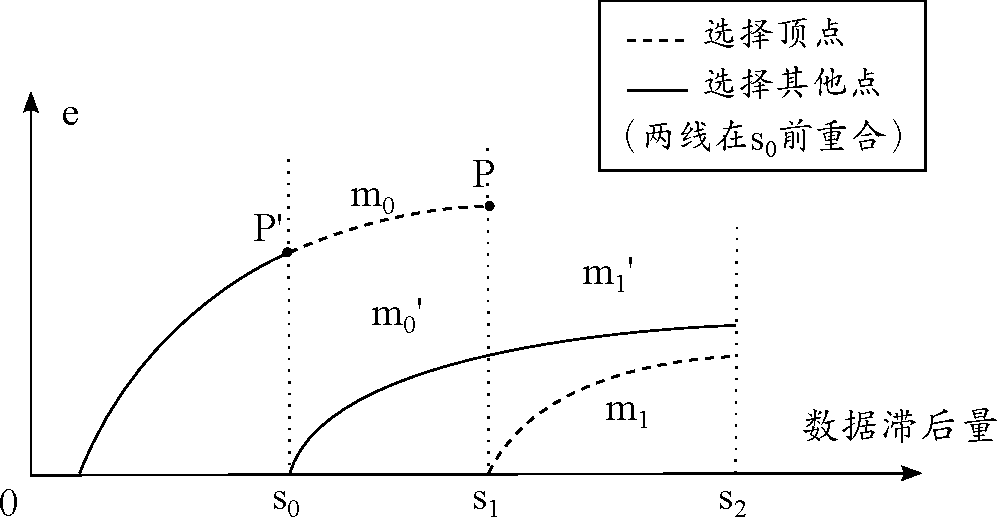
\includegraphics[width=0.7\textwidth]{tpl}
\caption{由选择不同的事务结束点产生的不同$e$曲线}
\label{fig:tpl}
\end{figure}

增加数据滞后量可以增加数据覆写的概率,从而节约数据冲刷量和相应的能耗,但付出的代价是更高的数据丢失的风险。所以我们面临这样的问题:MobiFS应该在多大程度上为减少能耗而增加数据滞后量?传统工作~\cite{Ma:2011:LPF:1989323.1989325, Mickens:2014:BFC:2616448.2616473, Ports:2010:TCA:1924943.1924963}仅通过设置一个较大的滞后量阈值来决定,而我们采用量化的动态的策略,依照每数据滞后量单元所节约的能耗量,即$e$比率(\ref{vct:insight}节)来决定。直观来看,$e$曲线的顶点是最佳权衡点,因为对应的能耗节约率最高。我们的设计原则是减少数据丢失风险,除非有特定的原因不这样做(为提升能量效率等)。 

具体地,我们提出最佳权衡点定位算法(tradeoff point location,TPL),用于确定写日志中结束当前事务的记录项。每个来自应用的写操作都会增加数据滞后量,对应于$e$曲线上的一个点。当一个事务关闭时,$e$曲线重新从$e=0$开始计算,如图\ref{fig:tpl}所示。最理想地,结束事务的最佳点应当在$e$值最高的曲线顶点。我们采用反证法,假设另一个算法决定在$P'$点关闭当前事务,此时$x = s_0$,而曲线顶点$P$处于不同的位置$x = s_1$。那么我们可以在保持下一个事务结束点$x = s_2$不变的前提下,通过将当前事务结束点变为$P$来获得更多的能耗节约量。将当前事务结束点由$P'$变为$P$可以提高数据覆写发生的概率\footnote{注意这不是一个严格的数学证明。虽然可以构造出反例,但总体来说可能性更大。}。不失一般性,我们令$s_0 < s_1$;在$[s_0, s_1]$($[s_1, s_2]$)区段,我们算法的覆写数据量为$m_0$($m_1$),假设的算法的覆写数据量是$m_0'$($m_1'$)。那么我们有$m_0 - m_0' > m_1' -
m_1$,原因如下:区段$[s_0, s_1]$上,$e$曲线仍然在快速上升,表明可以覆写的数据量较大,但却被假设算法截断,会导致大量可以覆写的数据丧失覆写机会;相反地,由于$P$是曲线顶点,如果不被截断,曲线在$[s_1, s_2]$区段上是下降的,意味着较少的数据可以被覆写。上述公式简单等价变换可得$m_0 + m_1 > m_0' + m_1'$。综上,在$P$点截断曲线是限制数据滞后量的一种手段,而采用我们的策略可以尽可能多地增加数据覆写的可能。
 
在实际中,我们还需要应对其他一些挑战。曲线会出现波动导致算法定位在局部最优解,为此我们使用一个滑动窗口进行线性拟合来屏蔽这些波动。具体地,算法记录$e$曲线上过去$k$个点,拟合出一条曲线,然后根据其斜率判断是否到达顶点。我们之所以选择线性拟合,而不是更高阶的曲线拟合,是因为策略引擎对于每次写操作都要进行计算,算法复杂度会影响CPU的能耗。与此同时,我们设置了一个数据滞后量(或者冲刷间隔时间)的上限,以防止为等待顶点出现而无穷等待的情况。该算法的评测参见\ref{vct:eval-ada}节。

\subsection{用户操作间隔预测}
\label{vct:interval}

间隔预测算法的主要目的是预测用户预期不进行操作的空闲间隔的时间长度。这些空闲间隔是适宜调度数据冲刷的时机。该算法一旦有VCT产生即被触发。为了评测该算法的有效性,我们把在预期没有操作的空闲间隔内意外发生的每次用户操作称为一个\emph{响应冲突}。注意一个预测的空闲间隔内可能遇到多个响应冲突。 
 
我们使用一个基于状态机的预测模型来平衡低响应冲突数(对响应度的负面影响低)和长预测间隔(潜在能量节约量大,因为更多VCT可在一个间隔内合并获得额外能量节约)。我们的算法是基于这样的观察:用户经常在短间隔和长间隔状态之间切换,例如,当浏览Facebook的新鲜事时,用户可能很快地跳过若干条目,然后停在一个感兴趣的内容上面阅读一定时间。注意本工作的定位不是给出一个完备的手机用户交互的模型,而是建立一个策略框架,并且展现我们使用的简单状态机模型的有效性。该模型可以满足我们的要求,有足够的能力学习用户的行为方式并做出高质量的预测(测评参见\ref{vct:eval-resp})。

图~\ref{fig-state-machine}描绘了我们的有限状态机模型。这里有两个中心状态:\textbf{\texttt{short interval}}(短间隔)态和\texttt{\textbf{long interval}}(长间隔)态,分别代表用户操作间隔较短和较长的情况。每个中心状态维护一个最近间隔的历史$A[1\ldots k]$,并使用其中最小的值$t$作为下一个间隔的预测。它们还各有一个计时器,用于必要时为超时事件设定时间。图中下标“s”和“l”分别表示这两个中心状态。与此同时,两个中间状态\texttt{\textbf{shorter interval}}态和\texttt{\textbf{longer
interval}}态,用于减少和增加间隔预期。

\begin{figure}[!h]
  \centering
  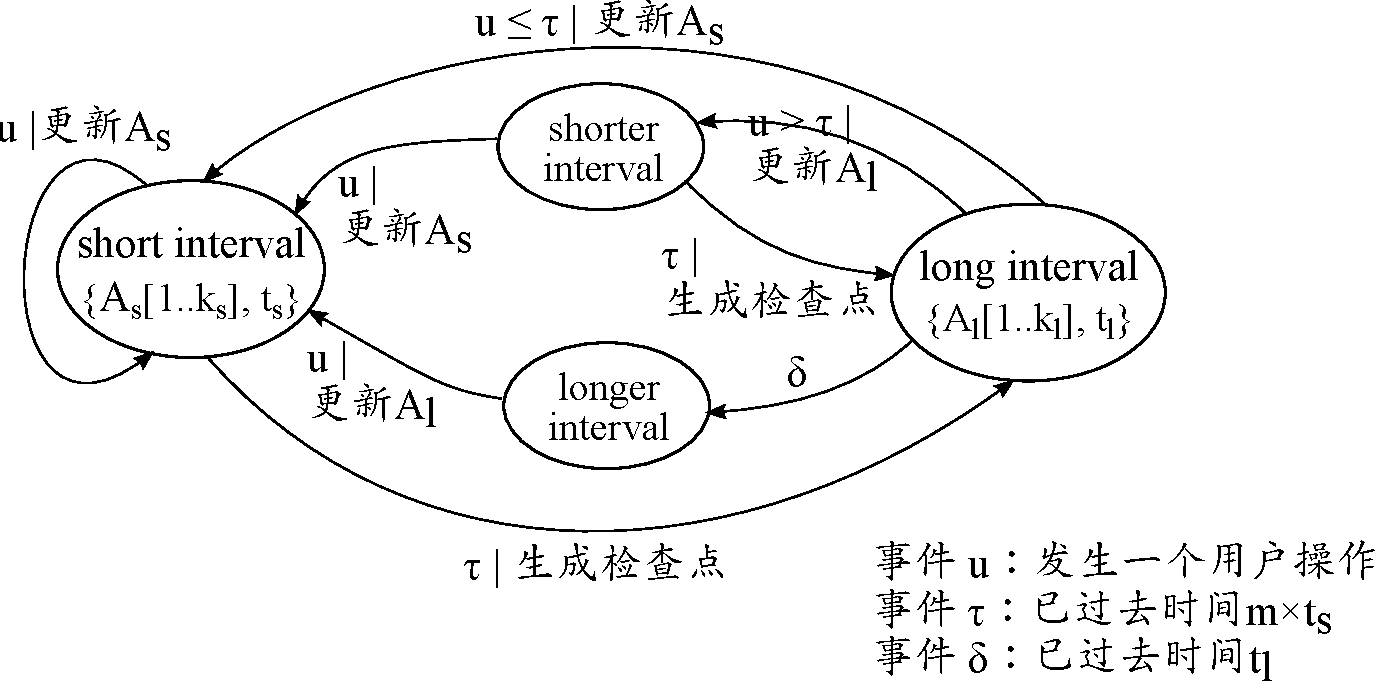
\includegraphics[width=\columnwidth]{state-machine}
  \caption{间隔预测算法的有限状态机}
  \label{fig-state-machine}
\end{figure}

直观上看,该状态机大体按如下的方式运转。当状态机处于\texttt{short interval}态的时候,如果首先到来的事件都是用户操作,它会一直不变状态地循环。但是,如果用户操作没有在超时事件
$\tau$(图~\ref{fig-state-machine})之前发生,状态机认为用户可能要开始一个长间隔,所以会转入\texttt{long interval}态。之后,如果预测间隔时间$t_l$内实际没有用户操作发生(即事件$\delta$),那么状态机进入\texttt{longer interval}态,并一直等到用户操作发生;否则,在\texttt{long interval}态时,如果用户操作晚于事件$\tau$,我们认为用户还处在长间隔的情况但是间隔的预测值应当下调,所以状态机进入\texttt{shorter interval}态,而如果用户操作很快发生(先于事件$\tau$),我们则猜测用户即将转入短间隔的状态,所以状态机直接进入\texttt{short interval}态。


\subsection{事务调度}
\label{vct:sched}

当一个用户与多个应用交互或者在各个应用间切换时,会出现事务调度的问题。一个典型的场景可能是用户玩手机游戏的同时在听音乐,而后台进程定期帮助用户检查电子邮件。此时,MobiFS可能会有多个写日志要提交各自(多个)已关闭的事务。我们的调度器需要为要生成检查点的VCT定序,并平衡应用响应度、能量效率和应用间公平性等因素。具体地,我们的算法考虑如下三个方面做出决定:(1)事务的长度,或者说要生成检查点的数据页的个数;(2)事务的相关性,同一个应用的各个事务间的相关性高,因为它们可以合并从而带来额外的能量节约;(3)事务的年龄,即该VCT之前已经跳过多少个可用间隔而没有被调度器选中刷出。 
 
我们采用基于优先级的调度算法,包含下面列出的四个按地位由高到低排序的规则。该算法维护了三级队列,每级队列保存相同年龄的一组事务。这些队列在被选择冲刷时会有不同的优先级。当一个VCT被调度选中时,来自相同应用的其他VCT会获得最高优先级。为讨论方便,我们不妨在下文直接使用应用作为描述调度策略的单位。

\begin{enumerate}
\item \textbf{规则1(事务相关性):}每当调度算法跳过了一个应用,这个应用即被移动到下一级更高优先级的队列上(如果该级队列存在)。

\item \textbf{规则2(事务年龄):}各个应用首先排入最低优先级的队列里,然后按照规则1逐步提升到高优先级的队列。当调度算法在所有优先级队列中都找不到可行的选择时,会选择最高优先级队列中长度最短的VCT实施检查点生成。

\item \textbf{规则3(事务长度):}队列中的一个应用可被选择生成检查点,仅当它首个VCT的长度预期的冲刷时间比当前预测的间隔时间短(即预期该次冲刷不会影响用户操作)。

\item \textbf{规则4(队列补充):}如果一个被选中的应用无法在当前可用间隔时间内生成所有VCT的检查点,那么剩余无法刷出的VCT移到最低优先级的队列中。

\end{enumerate}

\section{系统实现}

我们在Android 4.1(Linux 3.0.31)上实现了完全可用的原型系统,并分别与文件系统Ext4~\cite{Mathur:Ext4:2007}和Btrfs~\cite{Rodeh:2013:BLB:2501620.2501623}进行了整合。我们的实现包含
1996行C语言代码(不包括重用Ext4或Btrfs的组件)。MobiFS部署时不需要重新编译内核。

\subsection{主要组件}
\label{vct:data-struct}

\subsubsection{写日志}
我们使用循环数组实现写日志,因为它可以很好地支持需要的排序操作。为了节省空间,每个日志项的部分逻辑域(例如页索引和版本号)可以压缩到相同的物理域中。写日志内嵌一个\texttt{kobject}数据结构,使得MobiFS可以在\texttt{/sys}目录下导出可供用户态程序访问的配置接口,以方便配置。另外,日志上的操作可以支持适度的并行性,通过区分检查点生成操作和日志追加操作的区分实现——循环日志尾由一个自旋锁(spin lock)保护,而日志头由一个互斥量(mutex)保护,它只在日志尾触及日志头的时候用于排斥写操作。最后,为了定位哪个日志涵盖特定的文件,我们在该文件\texttt{inode}数据结构的\texttt{i\_private}域记录日志的编号。当一个新的文件生成时,它的\texttt{i\_private}值继承自它所在的目录。

\subsubsection{页逆向映射} 
一种实现页逆向映射的方式是在内核\texttt{page}数据结构中添加一个引用指针。然而\texttt{page}数据结构已经被填满(例如,超过24个标志挤在一个32位的域中),所以这种实现方式势必要扩大该数据结构的大小,而该数据结构对应于每个内存中的页,即便添加一个域也会带来可观的空间占用。与此不同,我们使用一个改造的哈希表结构来实现逆向映射的存储。该哈希表使用多个读写锁分别保护每个桶,而不是仅用一个全表的锁。我们增加与这些映射关联的页的\texttt{\_count}域值,使得现有Linux页缓存的实现不会把这些页收回。这也意味着MobiFS必须在内存空间不足时解除对这些页的锁定,让内核回收不用的页以释放内存空间。

\subsubsection{检查点生成器}
检查点生成器是一个内核线程。该线程在没有VCT要生成检查点时处于睡眠状态。当被策略引擎唤醒时,它首先在最近记录的用户交互历史上执行间隔预测算法,然后根据VCT调度策略,找到合适的VCT实施检查点生成。

\subsubsection{策略引擎}
策略引擎的实现需要考虑内核的诸多限制。例如,内核考虑FPU寄存器的开销,不直接支持浮点运算。因此,我们只能把$e$的值扩大$10^3$倍再用于我们的最佳权衡点定位算法,从而保持原数值千分位的精度。

\subsubsection{用户交互日志}
我们在一个队列中记录屏幕事件。一个特别的细节是,某些单个的逻辑用户操作(例如拖拽)会对应于很多个连续的间隔很小($<$ 0.01 ms)的物理事件。所以,我们需要一个过滤器来将这些事件合并成单一的用户操作。

\subsection{与现有存储组件的整合}
\label{vct:ext4}

我们的原型系统重用现有文件系统的组件实现其闪存管理和I/O功能。为了支持持久性和原子性事务,我们主要采用两种方法:预写式日志(write-ahead logging,WAL)和写时拷贝(copy-on-write,COW)。Ext4和 Btrfs分别是使用两类方法的典型的文件系统。

\subsubsection{Ext4}
Ext4使用WAL来实现持久性和原子性的事务。所有文件写操作首先被记入一个独立的日志区,而后再被移动到闪存主数据中。MobiFS与Ext4的结合需要考虑这种日志方式固有的双重写(write-twice)问题,即文件系统所有要写入闪存的数据实际都会被写入两遍。这可能会抵消MobiFS覆写优化节省的数据写入量。幸运的是,实际实验结果表明,MobiFS仍然可以实现显著的能量节约。

\subsubsection{Btrfs}
Btrfs依赖COW来实现持久性和原子性的事务。与WAL类似,COW不直接在闪存的目标数据上实施更改,而是首先生成目标数的一份新的副本,然后在该副本上进行修改,最后替换原有数据。虽然理论上Btrfs预期应该有更高的性能,但该文件系统的实现尚处于实验阶段,实际测试的表现并不理想。因为这样的原因,我们MobiFS整合Btrfs的实现(Btr-MobiFS)不如与Ext4的整合成熟。

\section{系统评测}
\label{vct:eval}

我们主要通过三个指标评价MobiFS的效能:对应用及用户的动态适应性(第\ref{vct:eval-ada}节),应用的响应度(第~\ref{vct:eval-resp}节),以及能量消耗(第\ref{vct:eval-energy}节)。在讨论系统设计带来的好处之前,我们也估计了MobiFS运行各个应用带来的额外内存开销(第\ref{vct:mem-fp}节)。

\subsection{评测方法} \label{vct:method}

我们的评测结果既包含基于日志的模拟,也包含实际设备上的测量;既包含基准测试集,也包含实际的应用。
我们使用一台三星手机Samsung
Galaxy Premier I9260(双核1.5~GHz处理器,1~GB内存,Android 4.1操作系统),和两个Kingston microSD闪存卡(默认的128~MB日志和4~KB块大小)。所有实验结果都在这两个崭新的闪存上重复,以避免硬件问题。
一台Monsoon电源监视器~\cite{Monsoon:PM}用于测量设备的能量消耗。默认情况下,MobiFS指我们基于Ext4的实现;文件系统Ext4使用默认的Android上的配置,仅通过日志保护元数据。

模拟用的日志收集自5位志愿者用户,他们每人各自操作了如下几款最为流行的应用(使用它们各自的私人账户登录):Facebook
(FB)、Pandora(PA)、Angry Birds(AB)、Netflix(NF)、Twitter(TT)、Google Maps(GM)、Citrix Receiver(CR)、Flipboard(FL)、Web Browser(WB)和WeChat(WC)。 每个应用的使用时间为5分钟。收集的日志包括I/O系统调用,页缓存访问和屏幕接触操作的时间戳。

基准测试集包含如下几个部分:(1)AnTuTu的I/O和数据库基准测试集;(2)RL面向SQLite的基准测试集,包含13个负载;(3)MobiBench基准测试集,主要模拟了Android系统的I/O特性。此外,我们还使用了一个自制的基准测试程序,它的主要行为是向一个文件的相同的区域顺序地通过\texttt{write}系统调用写入8~MB数据,重复该行为16遍,并在每2遍之后调用一次同步的\texttt{fsync}。

对于另一部分用代码操纵真实应用的实验,我们选择了浏览器、Facebook和Twitter三款应用,因为他们代表了三类典型的I/O特性:浏览器极少调用\texttt{fsync},其效能主要受Ext4文件系统后台冲刷的影响;Twitter与之相反,每秒钟发出高达50次以上的\texttt{fsync}系统调用;Facebook则发出中等数量的\texttt{fsync}系统调用。我们使用monkeyrunner~\cite{Monkeyrunner}来重现编码好的用户交互行为,以获得可重现性和可比性。我们使用局域网内的Apache2网页服务器测试浏览器,通过802.11n Wi-Fi连接,以尽量减小动态的网络状况对测试带来的噪音。

\subsection{内存开销} \label{vct:mem-fp}

我们依据I/O日志估计了MobiFS最坏情况下的内存开销,如图~\ref{fig:mem-fp}所示。
我们假设MobiFS不生成VCT的检查点。图中y轴是由文件系统引入的平均内存开销\footnote{为了反映各个内存开销曲线的不同形状,我们使用积分计算该均值。对于目标增长速率
$\alpha$以及已知的内存开销曲线在时间区段${\Delta t}$上的积分$I$,我们认为$\frac{1}{2}\alpha{\Delta t}^2 = I$,所以有
$\alpha=2I/{\Delta t}^2$。}的增长速率。平均而言,Ext4文件系统的开销在无操作系统干预的情况下以25.6~KB/s速率增长,而MobiFS导致的增长速率为35.8~KB/s。换句话说,如果有100~MB额外内存空间,MobiFS在最坏情况下可以支持一个应用运行17.4分钟而不冲刷数据到闪存(最坏情况的增长速率为100.5~KB/s)。需要注意的是,当内存开销超过一定阈值,MobiFS可以显式地执行检查点生成以释放内存占用。总之,考虑到对于应用而言设备内存日益充裕,MobiFS带来的内存开销是可以接受的。

\begin{figure}[!ht]
  \centering
  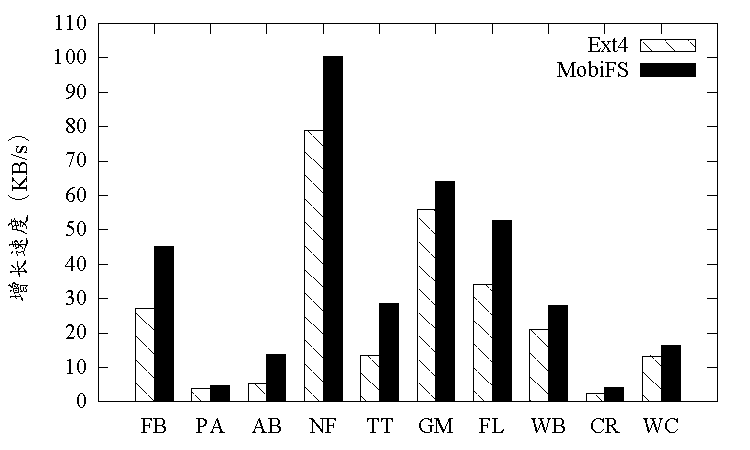
\includegraphics[width=\textwidth]{mem-fp}
  \caption{Ext4文件系统和MobiFS其上运行不同应用时的内存开销增长速率。}
  \label{fig:mem-fp}
\end{figure}

\subsection{对应用和用户的动态适应性} \label{vct:eval-ada}

本节测评MobiFS对于应用和用户的动态适应性。该适应性由我们的最佳权衡点定位算法实现(第\ref{vct:point}节)。

\noindent\textbf{对应用和用户的动态适应性:}
我们在I/O日志上执行最佳权衡点定位算法,并假设系统不考虑用户交互行为而立即生成检查点。
图\ref{fig:ada-int}展示了计算出的每个应用的平均检查点间隔。我们可以看到,MobiFS的平均检查点间隔有非常大的波动,其变化跨度可以达到21.7倍。与此同时,MobiFS几何平均的检查点间隔是普通Ext4冲刷间隔的17.5倍。MobiFS不仅大幅度扩展了Ext4冲刷的间隔,而且针对不同应用具有自适应性。

\begin{figure}[!ht]
  \centering
  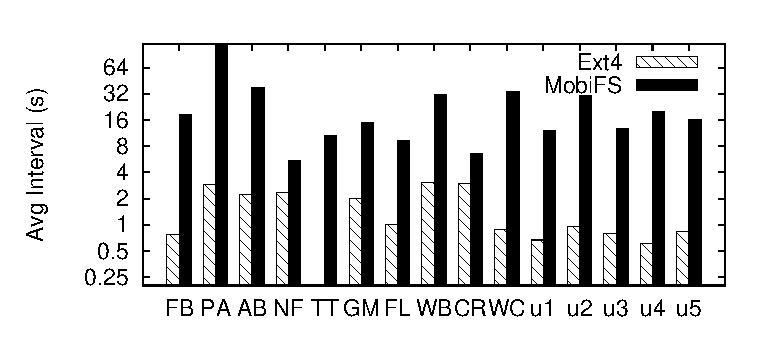
\includegraphics[width=\textwidth]{ada-int}
  \caption{MobiFS对于不同应用和用户产生的动态的检查点间隔。右侧用户统计数据(u$x$)基于用户使用Facebook的结果。}
  \label{fig:ada-int}
\end{figure}

图\ref{fig:ada-int}同时显示了Facebook的数据按用户聚类的平均检查点间隔。对于该单一应用,不同用户之间,仍体现出高达2.6倍的差异。这种面向用户的适应性是由于用户浏览的内容不同,内容的来源不同,以及个人操作习惯和阅读速度等方面的差异。

\noindent\textbf{自适应性带来的优势:}
假如我们完全不冲刷数据到闪存,那么此时的$e$曲线(称为理想化曲线)会呈现最大可能的数据覆写量。MobiFS通过适应不同的应用或用户个体,尽量贴近该理想化曲线。相比之下,Ext4文件系统则受限于固定的冲刷间隔和传统\texttt{fsync}系统调用的要求。为了展现MobiFS从自适应性中获得的好处,图\ref{fig:spa-ada}使用一个$e$曲线的变种来与Ext4文件系统比较。这里的$e$比率是基于从应用运行开始累积的总体数据滞后量$s$,而不像原定义中从上一次检查点算起。我们的获得的观察结论是,MobiFS更加紧密地跟进理想化曲线,而这里面体现的较高的数据覆写率代表着更好的能量效率。

\begin{figure}[!ht]
\centering
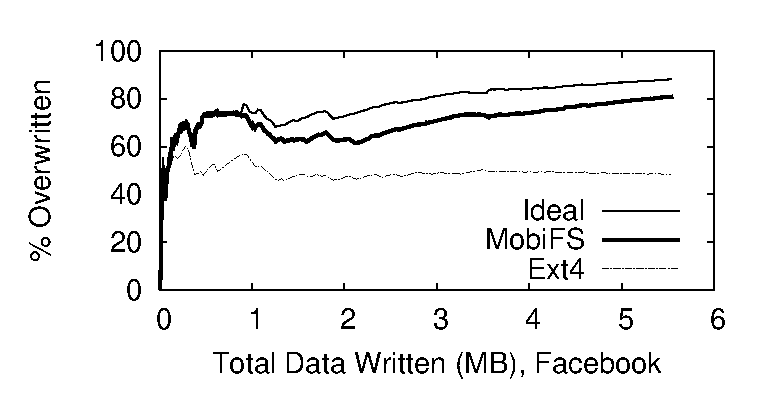
\includegraphics[width=\textwidth]{ada-facebook}\\
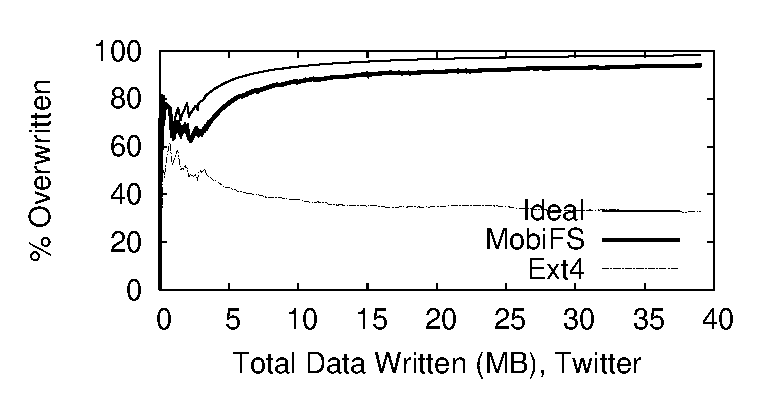
\includegraphics[width=\textwidth]{ada-twitter}\\
\caption{基于应用写数据累积量的$e$曲线。}
\label{fig:spa-ada}
\end{figure}

\subsection{应用响应度} \label{vct:eval-resp}

MobiFS聚焦在两个可以提升应用响应度的因素:尽量小的响应冲突,和尽量高的I/O效率。

\noindent\textbf{响应冲突:}
当我们的间隔预测算法(第\ref{vct:interval}节)预测了一个用户空闲间隔,MobiFS会尽量调度一次检查点生成操作来占满该段预测的空闲时间。响应冲突是指一个或多个预料之外的用户操作发生在了预期空闲的间隔内。我们用两个指标来评价预测的质量:(1)平均每次预测遇到的响应冲突;(2)预测间隔的平均时长。更长的间隔可以提供更多事务合并的可能,进而节省时间和能量消耗。

图\ref{fig:int-rc}和图\ref{fig:int-len}分别展示了MobiFS基于状态机的解决方案在上述两个指标上的表现。该结果依据我们的用户操作日志模拟得出。我们将MobiFS的方法与普遍使用的最近最小模型(last min model,LMM)和最近平均模型(last average model,LAM)进行比较。这两个模型分别使用最近$k$实际间隔的最小值或均值作为对下一个间隔的预测。由于LMM总是做出保守的选择,它仅造成每预测0.26次响应冲突,远小于LAM的1.18次。很自然,我们的状态机算法很难在这个指标上超越LMM,但实现了比LAM低54.8\%的表现。另一方面,LAM预测间隔的时长比LMM高很多。平均而言,我们的状态机算法可以达到LAM平均预测时长的75.9\%,而比LMM高出2.7倍。由于我们的状态机算法可以记忆之前的较长的间隔并据此信息做出预测,它甚至在9组应用测试中的3组上表现好于LAM。总结起来,MobiFS获得了接近于LMM的较低的响应冲突数,同时实现了类似于LAM的较长的预测间隔时长。它在LMM和LAM之间同时实现了双方的优势。

\begin{figure}[!ht]
  \centering
  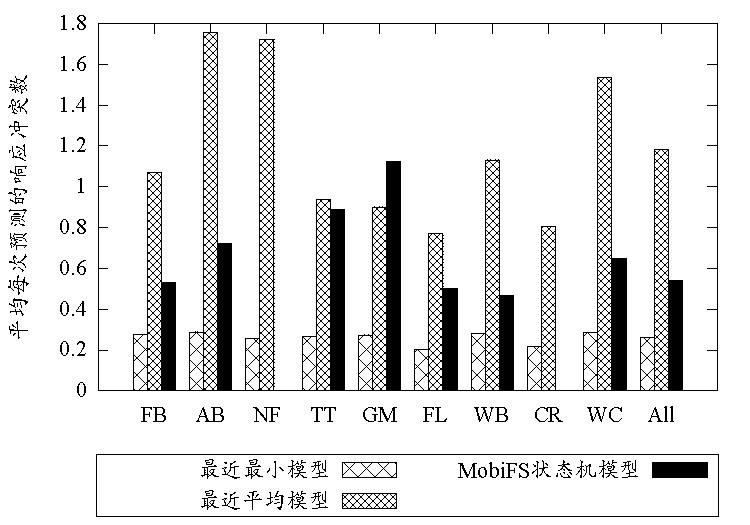
\includegraphics[width=\textwidth]{int-rc}
  \caption{三种模型的响应冲突比率。}
  \label{fig:int-rc}
\end{figure}

\begin{figure}[!ht]
  \centering
  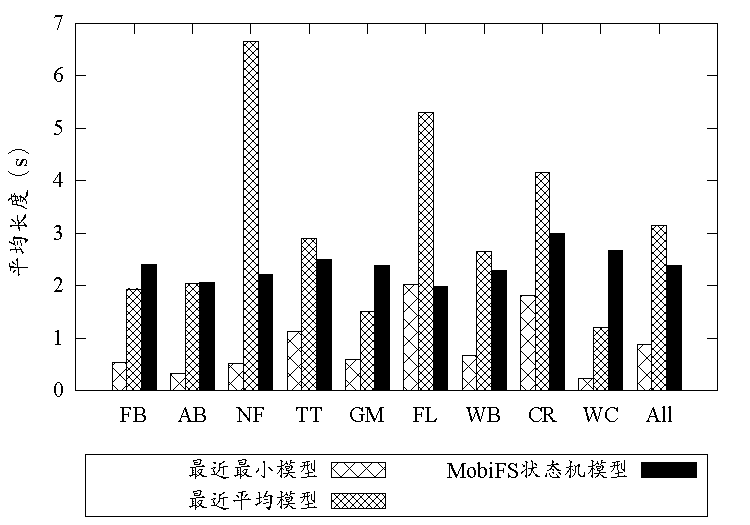
\includegraphics[width=\textwidth]{int-len}
  \caption{三种模型预测间隔的平均长度。}
  \label{fig:int-len}
\end{figure}

\noindent\textbf{I/O吞吐率:}
由于I/O在很大程度上影响应用的响应度,我们在实际设备上评测MobiFS在典型I/O指标上的表现。表\ref{tbl:micro-bench}和图\ref{fig:bench-item}显示了AnTuTu(ATT)、RL和MobiBench。结果表明,MobiFS的写性能可以超越Ext4高达480倍(例如随机写的结果),其上数据库操作的吞吐率也高出一个数量级。

\begin{table}[!ht]
\caption{在Android的Ext4和MobiFS上运行AnTuTu(ATT)和RL基准测试集获得的性能和能量数据。ATT的评分越高越好;RL基准测试集的执行时间越少越好。}
\label{tbl:micro-bench}
\begin{tabular}{p{0.45in}|p{0.45in}|*{2}{p{0.5in}}p{0.35in}}
 \hline
 \multicolumn{2}{c|}{项目} & Ext4 & MobiFS & 提升\\
 \hline
 \multirow{2}{*}{性能} & ATT评分 & 689.9$\pm$21.5 & 1817$\pm$51.0 & +163\% \\
 \cline{2-5}
 & RL(sec.) & 38.6$\pm$0.4 & 19.1$\pm$0.4 & -50.1\% \\
 \hline
 \multirow{2}{*}{能量(J)} & ATT & 24.3$\pm$0.8 & 20.3$\pm$0.7 & -16.4\% \\
 \cline{2-5}
 & RL & 43.8$\pm$0.5 & 37.6$\pm$0.6 & -14.2\% \\
 \hline
\end{tabular}
\end{table}

\begin{figure}[!ht]
  \centering
  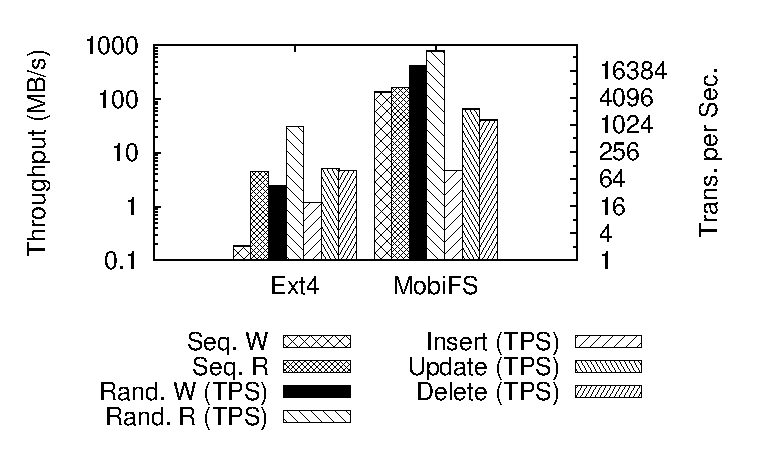
\includegraphics[width=\textwidth]{bench-item}
  \caption{MobiBench对Ext4和MobiFS的分项目性能测评。}
  \label{fig:bench-item}
\end{figure}

MobiFS倾向于挤压用于读的页缓存,因为Linux并不隔离用于读和写的缓存。幸运的是,根据我们的日志,平均有84.9\%的读操作可以命中在MobiFS锁定在内存的写缓存中。该现象缓解了读和写缓存不平衡的潜在问题。

\noindent\textbf{用户感知的延迟:}
我们通过测量monkeyrunner结束一段在实际设备上运行的预定义的用户交互过程的时间,来评价应用响应的延迟。这种方法的优势在于(1)可以消除真人用户操作中的随机性和不可比性以及(2)可以反应用户感知到的延迟而不包含真人用户具有差异的反应时间。在图\ref{fig:bench-app}中, monkeyrunner操作浏览器访问50个固定的网站,测得MobiFS上的平均页面载入时间比Ext4下降了49.0\%(平均每个操作减少延迟0.36秒)。对于Facebook采用类似方法,测得MobiFS上五次载入新鲜事的延迟相较Ext4下降53.6\%(平均每个操作减少延迟0.85秒)。最后,对于Twitter,载入\#Discover频道十次所需的时间在MobiFS上比Ext4下降了51.9\%(平均每个操作减少0.47秒延迟)。总之,MobiFS显著减小了真实应用上用户感知的操作延迟。

\begin{figure}[!ht]
  \centering
  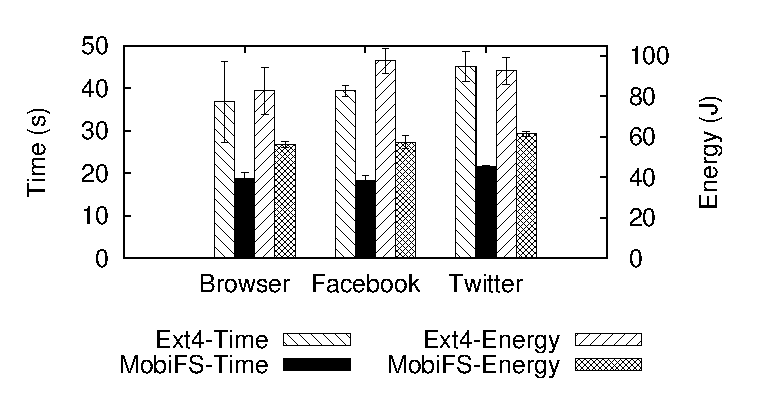
\includegraphics[width=\textwidth]{bench-app}
  \caption{在Android的Ext4和MobiFS上运行应用的响应度和能量消耗。}
  \label{fig:bench-app}
\end{figure}

\subsection{能量消耗} \label{vct:eval-energy}

MobiFS减少能量消耗的主要方式是减少冲刷到闪存的数据量。所以本节首先基于用户的日志模拟计算该数据量的减少,然后在实际设备上测量MobiFS的能量节约。

\noindent\textbf{刷出数据量的减少:}
图\ref{fig:flush-data}依据日志比较了Ext4和MobiFS刷出到闪存的数据量。节省的刷出数据量随各个应用有所不同,这依赖于一个应用发出的写中覆写的数量。取所有应用测试结果的几何平均,MobiFS比Ext4少刷出了53.0\%的数据量。

\begin{figure}[!ht]
  \centering
  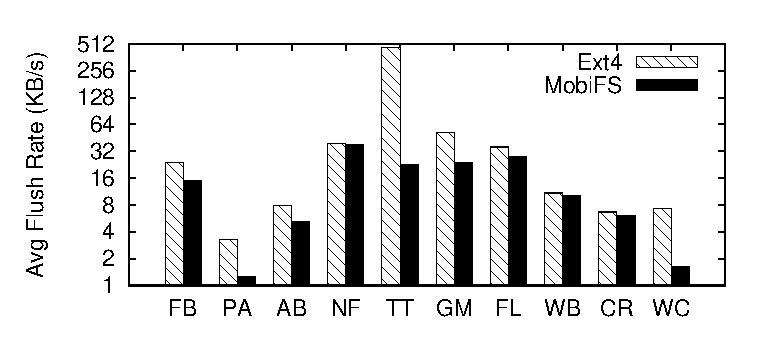
\includegraphics[width=\textwidth]{flush-data}
  \caption{在Android的Ext4和MobiFS上各个应用刷出的数据量。}
  \label{fig:flush-data}
\end{figure}

我们的评测表明MobiFS由于自身写两次的问题(第\ref{vct:ext4}节),刷出相同的数据量要比常规Ext4多花费66.4\%的能量。因此,总体上MobiFS模拟出的能量代价是Ext4的78.3\%。与此同时,如果我们计算所有应用刷出数据量的平均值,Ext4比MobiFS多刷出4.29倍的数据量,这意味着MobiFS比Ext4少消耗61.2\%的能量。

\noindent\textbf{设备能量节省:}
我们首先考虑图\ref{fig:baseline}中基准能量数据。逻辑上MobiFS只刷出Ext4一半的数据量,但由于写两次问题(第\ref{vct:ext4}节),理论上应当与Ext4有相似的能量消耗。然而在实际当中,Ext4模拟和原MobiFS需要的能量都比理论预期少(低16.8\%),因为内部的数据移动比显式地分开调用\texttt{write}节省CPU处理消耗。另一方面,尽管基于Btrfs的MobiFS实现“Btr-MobiFS”理论上没有写两次问题,但消耗的能量与Ext4类似,原因可能是COW及其自身实现的开销。另外,通过比较MobiFS和Ext4模拟,我们可以看到MobiFS特有组件的能量消耗只占总体的4.0\%。

\begin{figure}[!ht]
  \centering
  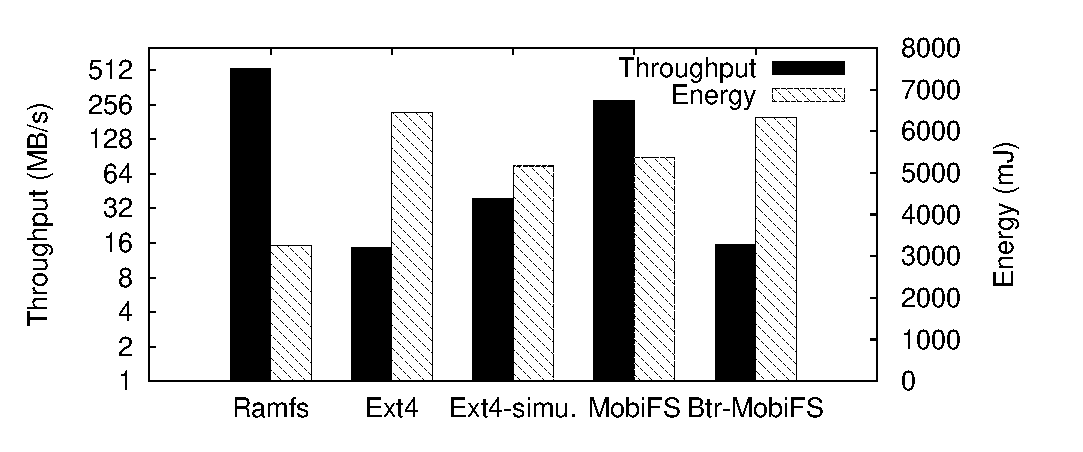
\includegraphics[width=\textwidth]{baseline}
  \caption{不同系统的基准测试程序结果。Ext4仅对元数据做日志;Ext4模拟是一个Ext4文件变形,模拟MobiFS的刷出行为,即在MobiFS刷出数据时也做刷出操作(对所有数据做日志)。}
  \label{fig:baseline}
\end{figure}

实际设备上运行基准测试集的结果也印证了MobiFS对减小能量消耗的贡献。表\ref{tbl:micro-bench}包含了AnTuTu和RL基准测试集下,MobiFS相对于Ext4的能量节约。值得注意的是,这些基准测试集的行为并没有完全体现出MobiFS可节约的全部潜能,因为我们的设计与应用和用户的行为高度适应。为此,我们采用真实应用和用户行为进行了下面的实验。

图\ref{fig:bench-app}比较了MobiFS和Ext4在真实设备上使用实际应用的能量代价。特别地,整体设备的能量代价在使用浏览器、Facebook和Twitter三种应用时分别平均下降了32.1\%、41.3\%和33.6\%。我们可以看到,MobiFS充分地提升了移动应用的能量效率。

\section{本章小结}

MobiFS在数据滞后—性能、数据滞后—能耗之间的权衡中,识别出一个本质上新的平衡点,成为新的手机文件系统设计的核心思想。它持久性内存假设和以内存为中心的设计理念,配合应用/用户感知的增量式检查点生成技术和支持异步\texttt{fsync}语义的多版本缓存事务技术,为下一代移动环境下数据存储设计提供了有益参考。在真实设备上使用实际用户日志、基准测试集和真实应用的评测显示,我们的策略设计有效并能够产生实际的效益。

